\subsection{Großtest 1:}\label{grosstest-1}

Die Handys wurden mit Buchstaben benannt und im Raum C205 verteilt.

\subsubsection{Ergebnisse Test 1:}\label{ergebnisse-test-1}

Wir haben auf 117 Nachrichten 11 erfolgreiche Fälle und 106 Errors.

\paragraph*{Folgende Beispiele veranschaulichen Nachrichten, die beim
Empfänger angekommen sind:}

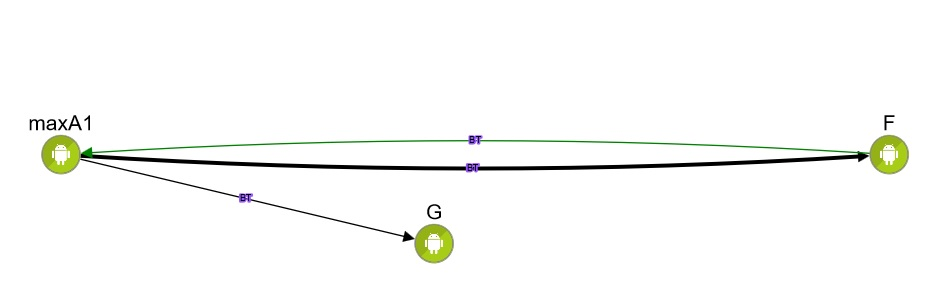
\includegraphics[width=1.0\textwidth]{belege/grosstests/Bilder/Erfolg4.jpg}\\
1. A sendet eine Nachricht an F. A sendet die Nachricht an G und F los, da A nur den
Bluetooth Namen der Handys kennt, und so nicht weiß, dass F sich in
Reichweite befindet. F sendet ein Acknowledgement zurück, während G die
Nachricht nicht weiterleiten kann.\\
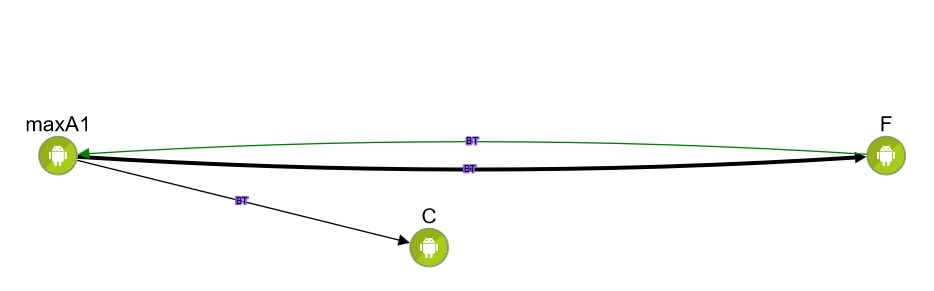
\includegraphics[width=1.0\textwidth]{belege/grosstests/Bilder/Erfolg3.jpg}\\
2. Gleiches Szenario wie in 2, nur diesmal mit C statt G.\\
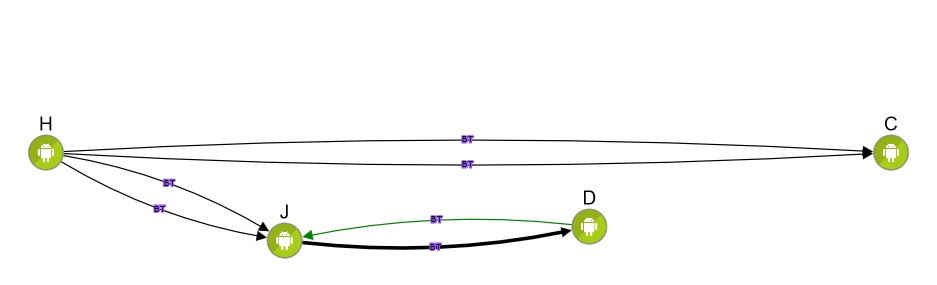
\includegraphics[width=1.0\textwidth]{belege/grosstests/Bilder/Erfolg2.jpg}\\ 3. H sendet eine
Nachricht an D. Es befinden sich J und C in Reichweite. C leitet die
Nachricht nicht weiter. J hat jedoch eine Verbindung zu D. D sendet ein
Acknowledgement über den Pfad, über den er die Nachricht empfangen hat
zurück.\\ 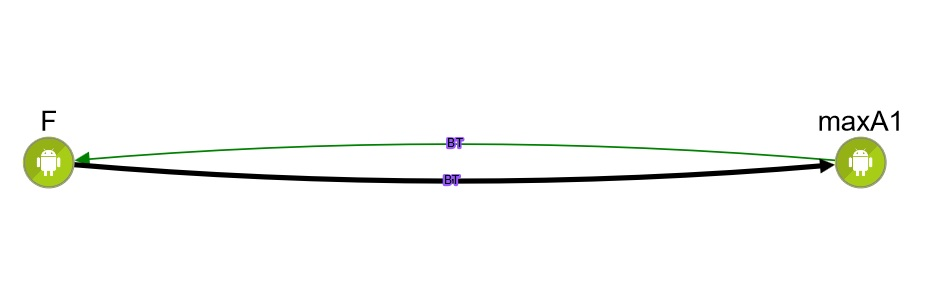
\includegraphics[width=1.0\textwidth]{belege/grosstests/Bilder/Erfolg1.jpg} \\4. Eine
Erfolgreich übertragene Nachricht zwischen 2 benachbarten Handys mit
Acknowledgement.

\paragraph*{Folgende Beispiele veranschaulichen Nachrichten, die nicht beim
Empfänger angekommen sind:}\\
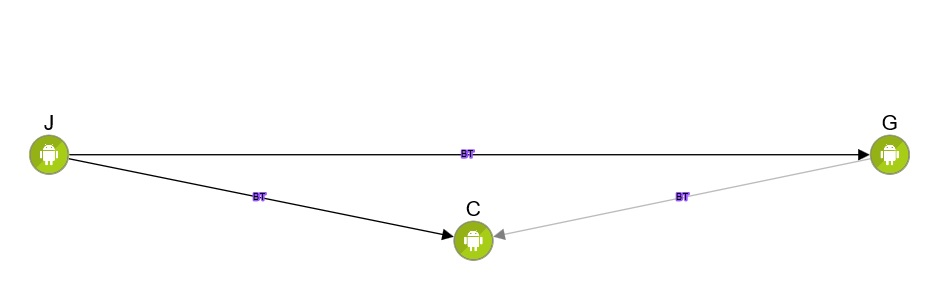
\includegraphics[width=1.0\textwidth]{belege/grosstests/Bilder/Miserfolg6.jpg}\\ 1. J versucht
eine Nachricht zu schicken. Es befinden sich jedoch nur die Handys G und
C in Reichweite. G kann daraufhin nur Verbindung mit C herstellen, das
jedoch die Nachricht bereits kennt.\\
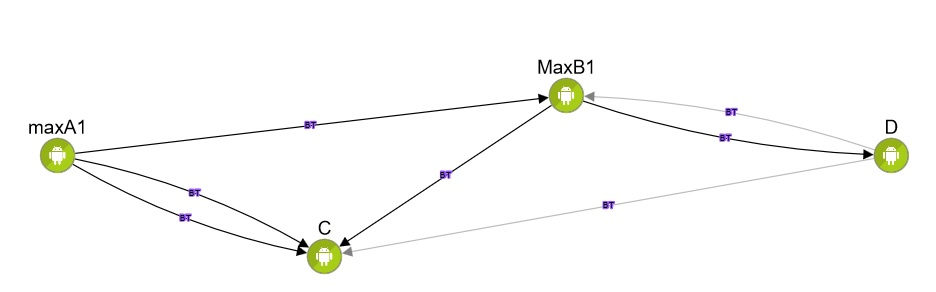
\includegraphics[width=1.0\textwidth]{belege/grosstests/Bilder/Miserfolg5.jpg}\\ 2. A versucht
eine Nachricht zu schicken. Es befinden sich jedoch nur die Handys B und
C in Reichweite. B kann die Nachricht nun noch an D weiterleiten. Dort
bleibt sie jedoch hängen, da D nur noch eine Verbindung zu C findet, das
die Nachricht bereits kennt. A versucht daraufhin in einem Retry die
Nachricht erneut zu schicken, findet aber nun nur noch C.\\
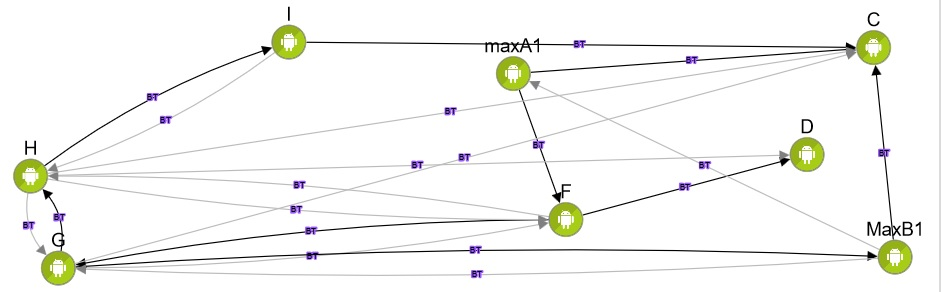
\includegraphics[width=1.0\textwidth]{belege/grosstests/Bilder/Miserfolg4.jpg}\\ 3. An diesem
Beispiel erkennt man, dass alle Handys nah zueinander lagen. Die
Nachricht wird von A verschickt. Sie durchläuft 7 der 9 anderen Handys.\\
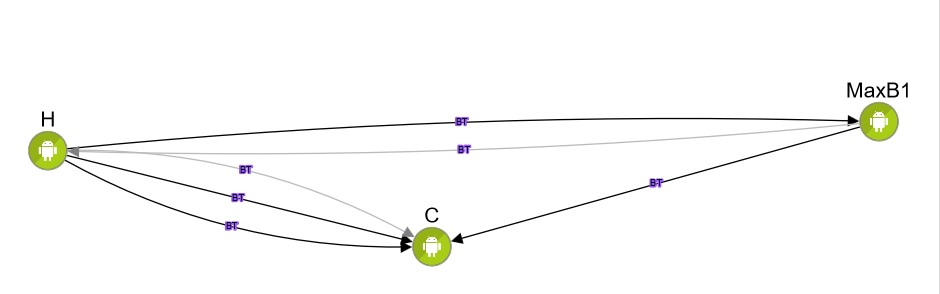
\includegraphics[width=1.0\textwidth]{belege/grosstests/Bilder/Miserfolg3.jpg}\\ 4. H versendet
diese Nachricht. Handy C blockiert jedoch die erfolgreiche Übermittlung
der Nachricht. \\
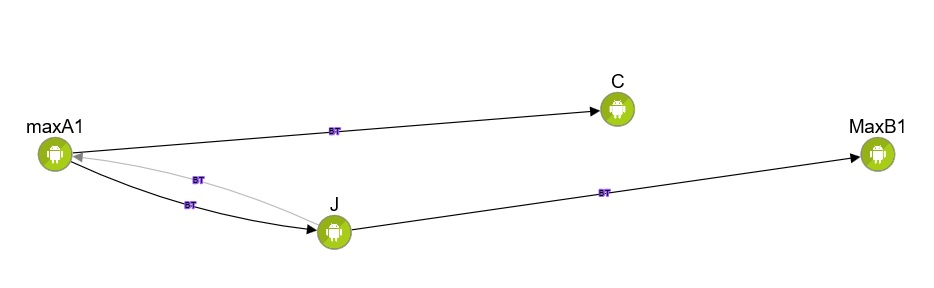
\includegraphics[width=1.0\textwidth]{belege/grosstests/Bilder/Miserfolg2.jpg}\\
5. Auch hier kommt die Nachricht nicht an Handy C vorbei. Auf einem
anderem Pfad schafft sie zwei Hops.\\
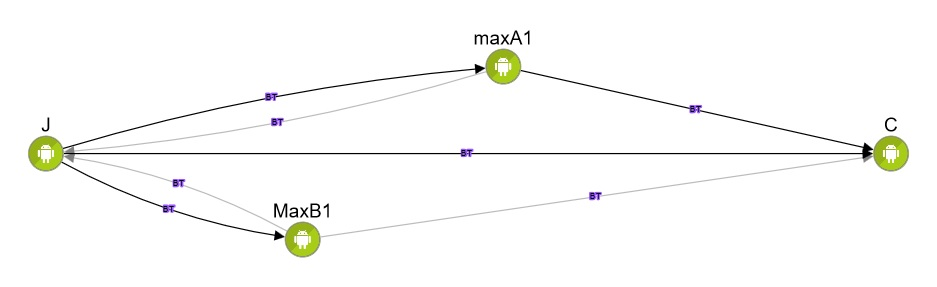
\includegraphics[width=1.0\textwidth]{belege/grosstests/Bilder/Miserfolg1.jpg}\\ 6. J versendet
hier die Nachricht an seine 3 Nachbarn. Da jedoch J, A und B (nur) C als
Nachbarn finden, kommt die Nachricht nicht an.\\

\subsubsection{Schlussfolgerung aus dem
Test:}\label{schlussfolgerung-aus-dem-test}

Es kamen extrem wenige Nachrichten an. Dies lag daran, dass die Handys
Probleme hatten, sich zu verbinden. Es liegt nahe, dass der
Bluetoothadapter nicht genügend Ports hat um sich mit allen in der Nähe
befindlichen Geräten zu verbinden. Eine Möglichkeit dies zu lösen, wäre
es, sich nicht dauerhaft mit allen Geräten in der Umgebung zu verbinden,
sondern eine Verbindung nach einer Übertragung wieder zu schließen.

Des Weiteren gab es Handys, die Nachrichten überhaupt nicht
weitergeleitet haben. Vermutlich war an diesen der Stromsparmodus von
Android aktiv. Ein Beispiel hierfür wäre C.

\paragraph*{Verbesserungen bis zum nächsten Test:}

\begin{itemize}
\tightlist
\item
  Die Anzahl der aufzubauenden Verbindungen heruntersetzen.
\item
  Ein Test mit mehr anwesenden Personen durchführen um Android daran zu
  hindern in den Stromsparmodus zu gehen, da dieser nicht ohne
  Root-Rechte abschaltbar ist.
\end{itemize}

\subsubsection{Ergebnisse Test 2:}\label{ergebnisse-test-2}

Bevor wir Test 2 gestartet haben, haben wir auf allen Handys den
Bluetooth Adapter deaktiviert und erneut aktiviert. Das sollte
eingefrorene Bluetooth Adapter wieder aktivieren. Dieses Vorgehen
basierte auf Erfahrungen von früheren kleinen Tests beim Programmieren.

Im Test 2 haben wir auf 166 Nachrichten 2 erfolgreiche Fälle und 164
Errors.

\paragraph*{Folgende Beispiele veranschaulichen die Nachrichten, die beim
Empfänger angekommen sind:}\\
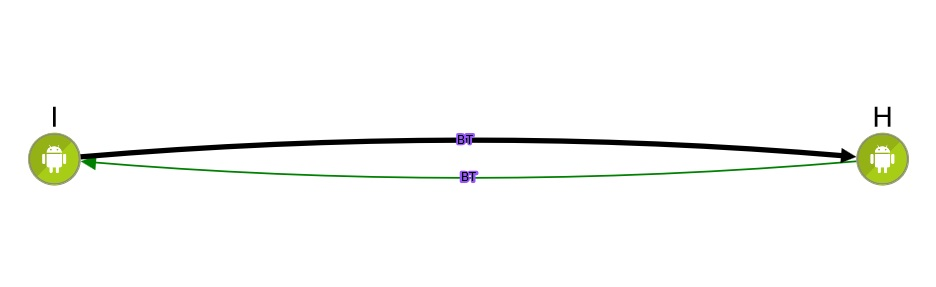
\includegraphics[width=1.0\textwidth]{belege/grosstests/Bilder/Test2Erfolg1.jpg}\\
 1. Nachricht
zwischen zwei benachbarten Handys.\\
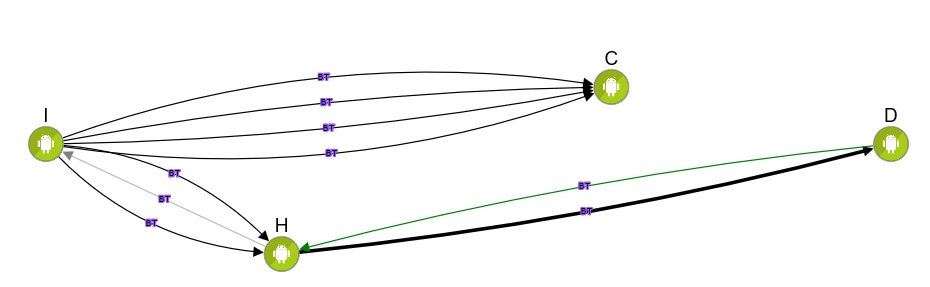
\includegraphics[width=1.0\textwidth]{belege/grosstests/Bilder/Test2Erfolg2.jpg}\\ 2. Nachricht
über einen Hop, die bei einem Retry erfolgreich wurde.\\

\paragraph*{Folgende Beispiele veranschaulichen Nachrichten, die nicht beim
Empfänger angekommen sind:}\\

\includegraphics[width=1.0\textwidth]{belege/grosstests/Bilder/Test2Misserfolg1.jpg}\\ 1. Das
Handy J hatte während des kompletten Tests keine Verbindung zu einem
Handy aufbauen können.\\
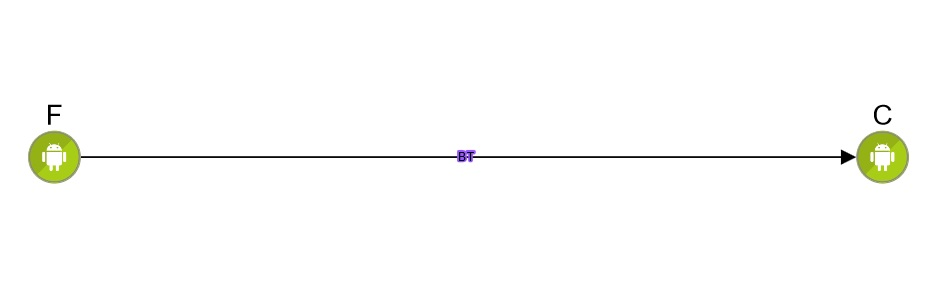
\includegraphics[width=1.0\textwidth]{belege/grosstests/Bilder/Test2Misserfolg3.jpg}\\ 2.
Generell hatten die Handys mehr Probleme Verbindungen aufzubauen.
Dadurch gab es viele Nachrichten, die gar nicht, oder nur bis zum
Nachbarn weitergeleitet wurden.\\
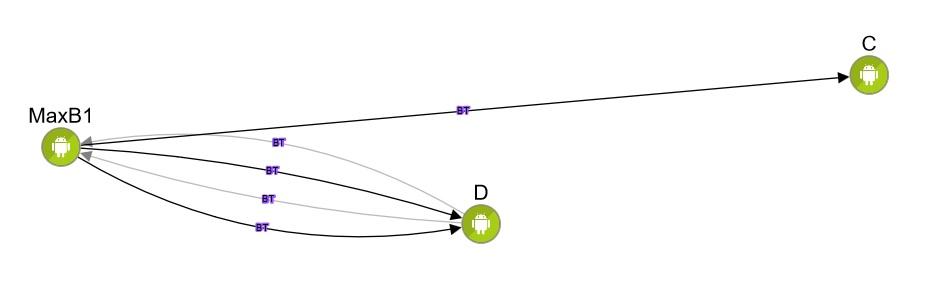
\includegraphics[width=1.0\textwidth]{belege/grosstests/Bilder/Test2Misserfolg4.jpg} \\3. Das
Handy B versucht eine Nachricht zu verschicken, schafft es jedoch nur
bis zu seinen unmittelbaren Nachbarn.\\
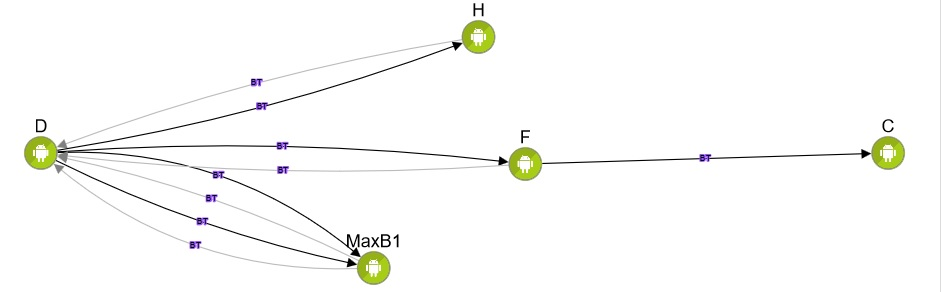
\includegraphics[width=1.0\textwidth]{belege/grosstests/Bilder/Test2Misserfolg5.jpg}\\
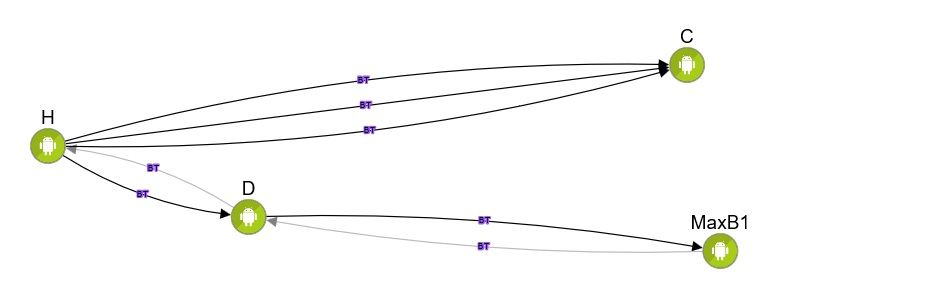
\includegraphics[width=1.0\textwidth]{belege/grosstests/Bilder/Test2Misserfolg6.jpg}\\ 4. und
5. Nachrichten wurden von einem Handy verschickt und schafften es eine
Nachricht mehr als einen Hop zu übertragen. Dies passierte bei diesem
Test bereits sehr selten.\\

\subsubsection{Schlussfolgerung aus dem
Test:}\label{schlussfolgerung-aus-dem-test-1}

Dieser Test zeigte, dass bereits Abstände von circa 5 Metern einen stark
beeinflussenden Faktor haben und extrem viel weniger Verbindungen
aufgebaut wurden als in Test 1.\\

Auch hier gab es wieder Handys, die vermutlich von Android in den
Energiesparmodus versetzt wurden, da diese von niemandem bedient wurden
und nur als Relaisstadion gedient haben.

\paragraph*{Verbesserungen bis zum nächsten Test:}

siehe Test 1, keine weiteren Erkenntnisse gewonnen.

\subsubsection{Test 3:}\label{test-3}

Da die Ergebnisse nicht unseren Erwartungen entsprachen, beschlossen wir
den Test hier abzubrechen. Der letzte Test unterliegt schwereren
Bedingungen und bringt dadurch nur bei Erfolg von Test 1 oder 2 bessere
Ergebnisse.

\subsection{Großtest 2:}\label{grosstest-2}

Nach dem letzten Test wurde der Code so erweitert, dass Bluetooth nur
noch 4 Verbindungen gleichzeitig aufbaut und in regelmäßigen Abständen
alte Verbindungen fallen lässt. Das hindert den Bluetooth Adapter zu
schnell zu überlasten.\\

Außerdem wurden weitere Kommilitonen darum gebeten am Test teilzunehmen.
Insgesamt wurde der Test von 9 Personen mit 14 Handys ausgeführt.\\

Die Benennung der Handys wurde den einzelnen Personen überlassen. Es
wurde dafür gesorgt, dass alle Handys den Kontakt der anderen Handys
kennt.\\

\subsubsection{Ergebnisse Test 1:}\label{ergebnisse-test-1-1}

Wir haben auf 167 Nachrichten 8 erfolgreiche Fälle und 159 Errors.

\paragraph*{Folgende Beispiele veranschaulichen Nachrichten, die beim
Empfänger angekommen sind:}\\
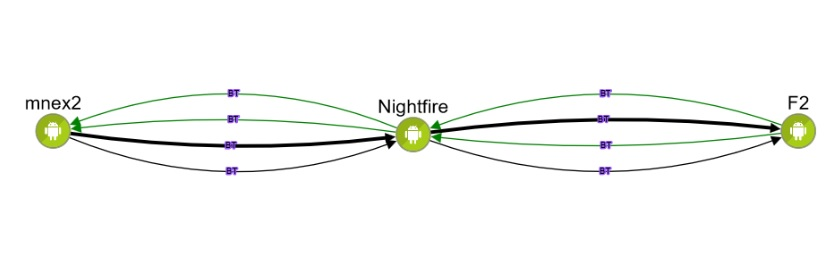
\includegraphics[width=1.0\textwidth]{belege/grosstests/Bilder/Grosstest2/Test1Erfolg2.jpg}\\
1. mnex2 sendet eine Nachricht an F2. Diese kommt erst nach einer
Retransmission an. Das Acknowledgement kommt auch erst beim 2. Versuch
an.\\
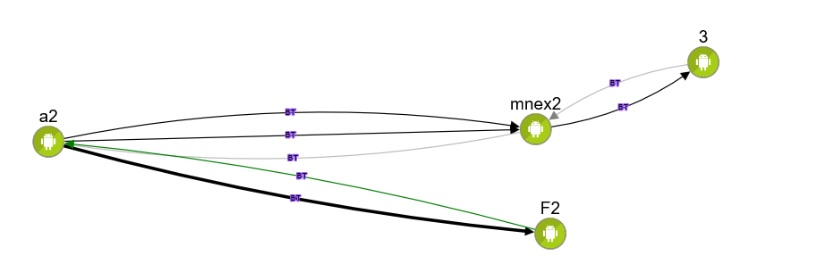
\includegraphics[width=1.0\textwidth]{belege/grosstests/Bilder/Grosstest2/Test1Erfolg1.jpg}\\
2. Hier sendet a2 eine Nachricht an F2. Da F2 ein Nachbar ist, kommt die
Nachricht direkt an. A2 versucht gleichzeitig auch noch einen weiteren
Weg, der jedoch nach einem Hop verloren geht.\\
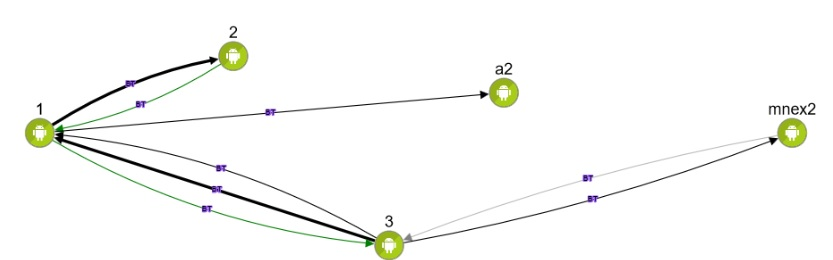
\includegraphics[width=1.0\textwidth]{belege/grosstests/Bilder/Grosstest2/Test1Erfolg3.jpg}\\
3. In dieser Nachricht sendet 3 an 2. Die Nachricht wird erfolgreich über 1
geschickt. 1 sendet die Nachricht gleichzeitig auch noch an a2.

\paragraph*{Folgende Beispiele veranschaulichen Nachrichten, die nicht beim
Empfänger angekommen sind:}\\
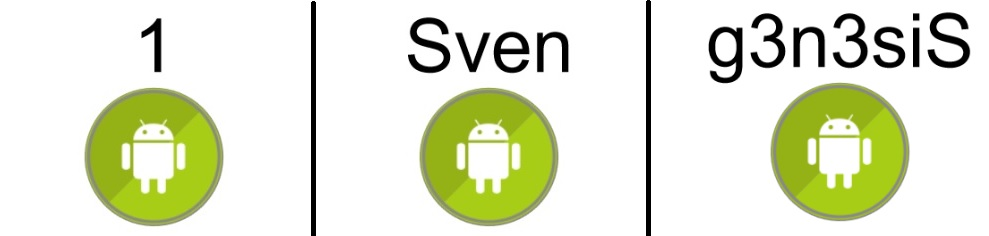
\includegraphics[width=1.0\textwidth]{belege/grosstests/Bilder/Grosstest2/Test1Misserfolg2.jpg}\\
1. Bei diesem Test kam es häufig zur Situation, dass Handys überhaupt keine
Verbindung mit anderen Geräten herstellen konnten. Dies kann daran
liegen, dass die Geräte in der Näheren Umgebung bereits 4 Verbindungen
offen hatten, oder dessen Bluetooth durch frühere Transmissions
überlastet war.\\

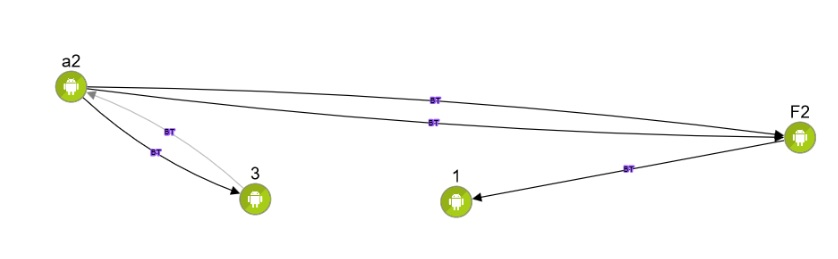
\includegraphics[width=1.0\textwidth]{belege/grosstests/Bilder/Grosstest2/Test1Misserfolg1.jpg}\\
2. Hier sendet a2 eine Nachricht, die jedoch nur über einen Hop
weitergeleitet wird und deshalb nicht ankommt.\\
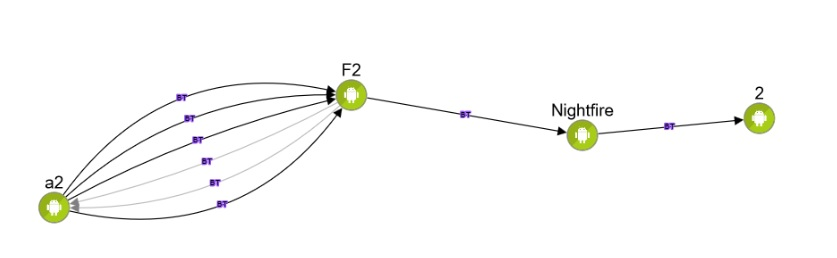
\includegraphics[width=1.0\textwidth]{belege/grosstests/Bilder/Grosstest2/Test1Misserfolg3.jpg}\\
3. Auch hier sendet a2 eine Nachricht, die über die Hops F2, Nightfire und
2 läuft, dort jedoch verloren geht.\\

\subsubsection{Schlussfolgerung aus dem
Test:}\label{schlussfolgerung-aus-dem-test-2}

Die Einschränkung auf 4 Verbindungen pro Bluetooth-Gerät scheint nicht
erfolgreich gewesen zu sein. Der Bluetoothadapter scheint immer noch
sehr schnell zu überlasten. Die Einschränkung führt außerdem noch dazu,
dass nicht alle Handys in der Umgebung erreicht werden, da bereits 4
Verbindungen bestehen, oder versucht aufgebaut zu werden.\\

Es bestand kein Grund zur Annahme, dass Verbindungen bei diesem Test
nicht zustande gekommen sind, weil ein Handy in den Standby Modus
gegangen ist.

\subsubsection{Ergebnisse Test 2:}\label{ergebnisse-test-2-1}

Wir haben auf 227 Nachrichten 20 erfolgreiche Fälle und 7 Errors.\\

\paragraph*{Folgende Beispiele veranschaulichen Nachrichten, die beim
Empfänger angekommen sind:}\\
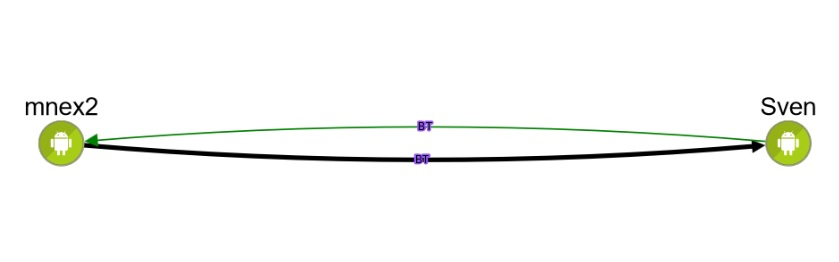
\includegraphics[width=1.0\textwidth]{belege/grosstests/Bilder/Grosstest2/Test2Erfolg1.jpg}\\
1. Die Verbindung zwischen mnex2 und Sven bestand über den ganzen Test.
Über diese Verbindung gingen 13 Nachrichten.\\
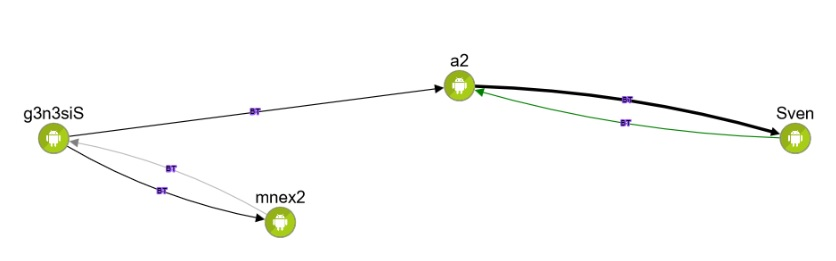
\includegraphics[width=1.0\textwidth]{belege/grosstests/Bilder/Grosstest2/Test2Erfolg3.jpg}\\
2. G3n3siS sendet eine Nachricht an Sven. Diese wird erfolgreich an a2
übermittelt, welches diese dann an Sven weiterleitet. Das
Acknowledgement kommt jedoch nicht mehr zurück.\\
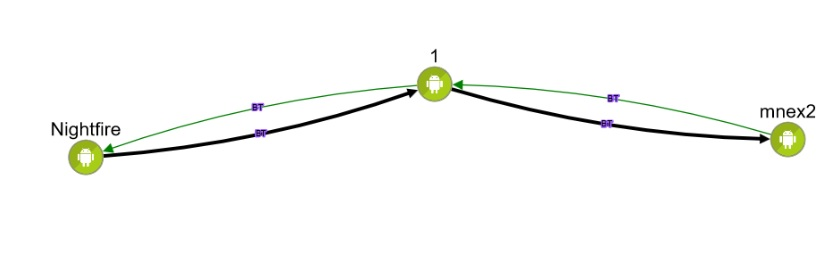
\includegraphics[width=1.0\textwidth]{belege/grosstests/Bilder/Grosstest2/Test2Erfolg4.jpg}\\
3. Nightfire sendet eine Nachricht an mnex2.\\

\paragraph*{Folgende Beispiele veranschaulichen Nachrichten, die nicht beim
Empfänger angekommen sind:}\\

\includegraphics[width=1.0\textwidth]{belege/grosstests/Bilder/Grosstest2/Test2Misserfolg1.jpg}\\
1. Im Verhältnis zu Test 1 gab es noch häufiger die Situation, dass Handys
gar nicht mit anderen Geräten verbunden sind.\\
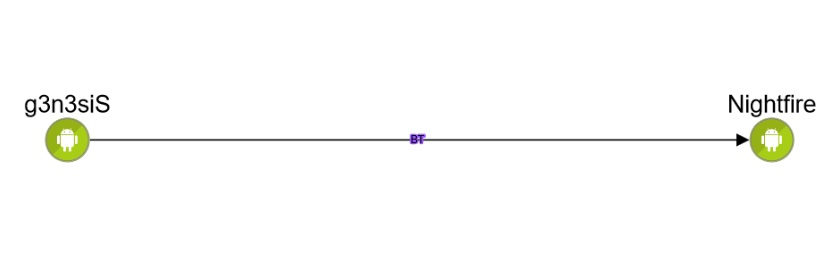
\includegraphics[width=1.0\textwidth]{belege/grosstests/Bilder/Grosstest2/Test2Misserfolg2.jpg}\\
2. G3n3siS verschickt eine Nachricht, die jedoch von seinem Nachbarn
Nightfire nicht weitergeleitet wird.\\
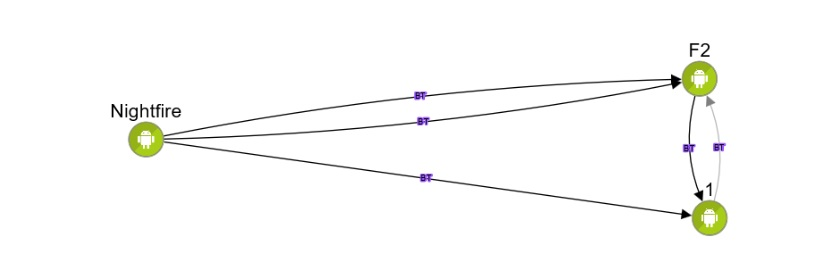
\includegraphics[width=1.0\textwidth]{belege/grosstests/Bilder/Grosstest2/Test2Misserfolg3.jpg}\\
3. Nightfire baut eine Verbindung zu mehreren Nachbargeräten auf, die sich
jedoch nur gegenseitig finden.\\

\subsubsection{Schlussfolgerung aus dem
Test:}\label{schlussfolgerung-aus-dem-test-3}

Die Anzahl der erfolgreichen Verbindungen ist sehr stark von der
funktionierenden Verbindung zwischen mnex und Sven beeinflusst.\\

Die Tatsache, dass extrem viele Geräte überhaupt keine Verbindung mehr
aufbauen konnten, unterstützt die Aussage, die bereits nach Test 1
getroffen wurde, dass die Limitierung der Slots nicht zielführend war.

\subsubsection{Ergebnisse Test 3:}\label{ergebnisse-test-3}

Da wir gemerkt haben, dass die Limitierung der Slots auf 3 nicht
zielführend war, haben wir diese für Test 3 wieder rückgängig gemacht.\\

Wir haben auf 164 Nachrichten 11 erfolgreiche Fälle und 153 Errors.

\paragraph*{Folgende Beispiele veranschaulichen Nachrichten, die beim
Empfänger angekommen sind:}\\
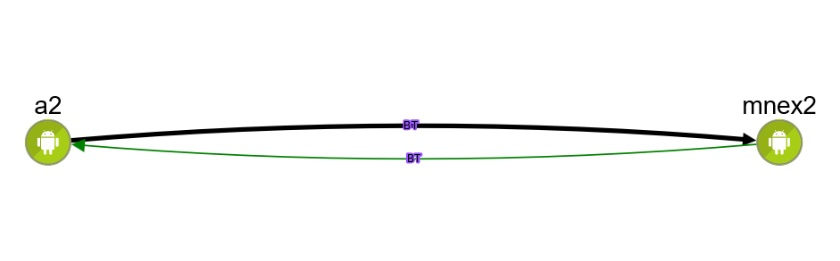
\includegraphics[width=1.0\textwidth]{belege/grosstests/Bilder/Grosstest2/Test3Erfolg1.jpg}\\
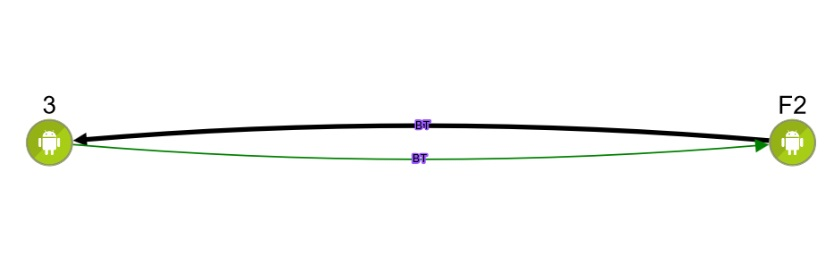
\includegraphics[width=1.0\textwidth]{belege/grosstests/Bilder/Grosstest2/Test3Erfolg2.jpg}\\
1 und 2. Nachrichten die zu einem benachbarten Empfänger gesendet werden.\\
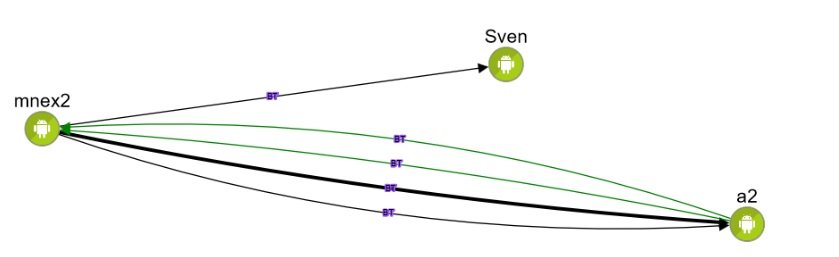
\includegraphics[width=1.0\textwidth]{belege/grosstests/Bilder/Grosstest2/Test3Erfolg3.jpg}\\

3. Mnex sendet eine Nachricht an Sven diese kommt jedoch erst nach dem
zweiten Versuch an. Auch das Acknowledgement benötigt 2 Versuche.

\paragraph*{Folgende Beispiele veranschaulichen Nachrichten, die nicht beim
Empfänger angekommen sind:}\\

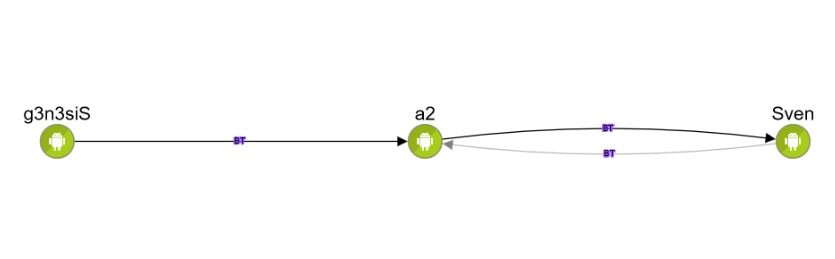
\includegraphics[width=1.0\textwidth]{belege/grosstests/Bilder/Grosstest2/Test3Misserfolg1.jpg}\\
1. G3n3siS sendet eine Nachricht. Diese geht jedoch nach 2 Hops verloren.\\

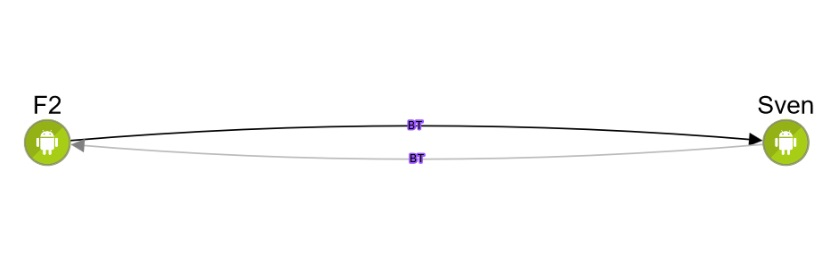
\includegraphics[width=1.0\textwidth]{belege/grosstests/Bilder/Grosstest2/Test3Misserfolg2.jpg}\\
2. Das wohl häufigste Beispiel des dritten Tests. 2 Benachbarte Geräte
schaffen es eine Verbindung aufzubauen. Das zweite Handy schafft es
jedoch dann nicht, die Nachricht weiterzuleiten.\\



\includegraphics[width=1.0\textwidth]{belege/grosstests/Bilder/Grosstest2/Test3Misserfolg3.jpg}\\
3. Auch hier gab es Fälle, in denen ein Handy keine Verbindung mit einem anderen Gerät aufbauen konnte. Dies passiert jedoch deutlich seltener als bei Test 1 und 2. \\
\subsubsection{Schlussfolgerung aus dem
Test:}\label{schlussfolgerung-aus-dem-test-4}

Der dritte Test ist besser gelaufen als der 2. Da die Entfernung einen
erschwerenden Faktor darstellt, kann davon ausgegangen werden, dass die
Verbesserung dadurch zustande kam, dass wir die Slots nicht mehr
limitieren.

\subsubsection{Ausblick und zukünftige
Tests:}\label{ausblick-und-zukuxfcnftige-tests}

Im Auftragsgebertreffen wurde entschieden, dass keine weiteren
Verbesserungen am Bluetoothcode durchgeführt werden sollen. Die Begründung
hierfür ist, dass die Implementierung des Bluetooth Stacks wohl
teilweise fehlerhaft ist.

Die Lösung hierfür ist eine eigene Implementierung des Bluetooth Stacks.
Diese soll jedoch im Rahmen einer Bachelorarbeit geschrieben werden, da
dies nicht Bestandteil des Bachelorpraktikums ist.

Da sich deshalb in der Funktionalität der Nachrichtenübertragung nichts
mehr ändern wird, haben wir auf den dritten Großtest verzichtet.
